% ==================================================================
% 3 METODOLOGIA
% ==================================================================

\chapter{METODOLOGIA}

\section{TIPO DE PESQUISA E ESTRATÉGIA METODOLÓGICA}

Este estudo é de natureza quantitativa, descritiva e comparativa, com foco na avaliação do desempenho de diferentes estratégias de alocação de ativos financeiros. A pesquisa adota uma abordagem empírica, utilizando dados históricos do mercado financeiro brasileiro para a construção e análise das carteiras.

\section{PERÍODO E AMBIENTE DE ESTUDO}

O horizonte temporal da análise compreende o período de janeiro de 2018 a dezembro de 2019, um momento de alta volatilidade e instabilidade política no Brasil. O ambiente de estudo é a B3 -- Brasil Bolsa Balcão, principal bolsa de valores brasileira.

\section{SELEÇÃO DOS ATIVOS}

A seleção dos ativos da amostra segue critérios rigorosamente \textbf{ex-ante}, baseados exclusivamente em informações disponíveis antes do período de teste (2018-2019):

\begin{itemize}
    \item \textbf{Alta liquidez histórica:} Volume médio diário de negociação superior a R\$ 50 milhões, calculado exclusivamente com base no histórico de janeiro de 2016 a dezembro de 2017;
    
    \item \textbf{Diversificação setorial:} Inclusão de ações de diferentes setores da economia brasileira;
    
    \item \textbf{Capitalização de mercado:} Empresas de maior valor de mercado em dezembro de 2017, geralmente pertencentes ao índice Ibovespa na época.
\end{itemize}

\textbf{Importante:} Esta metodologia de seleção elimina o survivorship bias, pois todos os critérios são baseados em informações anteriores ao período de teste. Não foi aplicado qualquer filtro baseado no desempenho ou sobrevivência durante 2018-2019, garantindo que a amostra reflita as decisões de investimento que poderiam ter sido tomadas em tempo real no início de 2018.

\subsection{Critérios de Seleção Final}

\begin{itemize}
    \item \textbf{Representatividade de mercado:} Preferência por empresas pertencentes ao índice Ibovespa em janeiro de 2018, garantindo representatividade do mercado brasileiro;
    
    \item \textbf{Diversificação setorial:} Máximo de 2 ativos por setor econômico, baseada na classificação setorial da Economática, visando reduzir riscos de concentração setorial;
    
    \item \textbf{Capitalização de mercado:} Ranking por valor de mercado em janeiro de 2018, priorizando empresas de maior porte dentro de cada setor selecionado.
\end{itemize}

Estes critérios visam evitar viés de sobrevivência (survivorship bias) e garantir que a amostra seja representativa do universo de investimentos disponível para gestores profissionais no início do período de análise.

\subsection{Distribuição Setorial da Base de Dados}

A base de dados da Economática apresenta a seguinte distribuição setorial entre as 508 empresas analisadas:

\begin{itemize}
    \item \textbf{Outros:} 117 empresas (23,0\%)
    \item \textbf{Energia Elétrica:} 65 empresas (12,8\%)
    \item \textbf{Finanças e Seguros:} 45 empresas (8,9\%)
    \item \textbf{Comércio:} 40 empresas (7,9\%)
    \item \textbf{Construção:} 33 empresas (6,5\%)
    \item \textbf{Siderurgia \& Metalurgia:} 32 empresas (6,3\%)
    \item \textbf{Demais setores:} 176 empresas (34,6\%)
\end{itemize}

A partir desta base, foram selecionados 10 ativos representativos, garantindo diversificação setorial e alta liquidez, conforme os critérios estabelecidos.

\subsection{Caracterização da Amostra Final}

A seleção final resultou em uma carteira diversificada de 10 ativos representativos do mercado brasileiro:

\begin{table}[H]
\centering
\caption{Ativos Selecionados para Análise}
\begin{tabular}{llllc}
\toprule
\textbf{Código} & \textbf{Empresa} & \textbf{Setor} & \textbf{Subsetor} & \textbf{Peso Ibov 2018} \\
\midrule
PETR4 & Petrobras & Petróleo e Gás & Exploração & 8,2\% \\
VALE3 & Vale S.A. & Mineração & Minério de Ferro & 14,1\% \\
ITUB4 & Itaú Unibanco & Finanças e Seguros & Bancos & 6,3\% \\
BBDC4 & Bradesco & Finanças e Seguros & Bancos & 4,8\% \\
ABEV3 & Ambev S.A. & Bebidas & Cervejas & 4,1\% \\
B3SA3 & B3 S.A. & Finanças e Seguros & Serv. Financeiros & 2,9\% \\
WEGE3 & WEG S.A. & Máquinas e Equipamentos & Motores & 2,1\% \\
RENT3 & Localiza & Outros Serviços & Aluguel Veículos & 1,8\% \\
LREN3 & Lojas Renner & Comércio & Varejo Vestuário & 1,4\% \\
ELET3 & Eletrobras & Energia Elétrica & Geração & 0,9\% \\
\bottomrule
\end{tabular}
\label{tab:ativos_selecionados}
\end{table}

\subsection{Justificativa da Seleção}

Esta composição garante:
\begin{itemize}
    \item \textbf{Diversificação setorial:} 7 setores distintos representados
    \item \textbf{Representatividade:} 46,6\% do peso total do Ibovespa em janeiro de 2018
    \item \textbf{Liquidez:} Volume médio diário superior a R\$ 100 milhões para todos os ativos
    \item \textbf{Capitalização:} Empresas de grande porte com histórico consolidado
    \item \textbf{Sobrevivência:} Todos os ativos mantiveram negociação ativa durante 2018-2019
\end{itemize}

\section{COLETA E TRATAMENTO DOS DADOS}

Os dados históricos de preços ajustados dos ativos foram coletados da base de dados Economática, abrangendo o período de 2014 a 2019. A base contém informações detalhadas de 508 empresas listadas na B3, incluindo:

\begin{itemize}
    \item \textbf{Dados de cotações:} preços de abertura, fechamento, máximo, mínimo e médio, todos ajustados por proventos (dividendos, juros sobre capital próprio, bonificações e desdobramentos);
    \item \textbf{Volume de negociação:} quantidade de negócios, títulos e volume financeiro;
    \item \textbf{Classificação setorial:} setor Economática, setor econômico Bovespa e segmento Bovespa;
    \item \textbf{Códigos dos ativos:} identificação única de cada papel negociado.
\end{itemize}

A utilização de preços ajustados por proventos é fundamental para evitar distorções na análise de retornos, uma vez que eventos corporativos como dividendos causam quedas artificiais nos preços das ações na data ex-dividendo. Sem esse ajuste, os retornos calculados seriam inconsistentes e não refletiriam a performance real dos investimentos.

O tratamento dos dados inclui:

\begin{itemize}
    \item Remoção de ativos com dados faltantes ou séries históricas incompletas no período de análise;
    \item Cálculo dos retornos mensais e anualizados com base nos preços de fechamento ajustados;
    \item Estimativa das volatilidades individuais e matriz de covariância entre os retornos dos ativos;
    \item Definição da taxa livre de risco como o CDI médio anualizado do período: $(6,43\% + 5,96\%)/2 = 6,195\%$ a.a., com base em dados oficiais do Investidor10 (fonte: B3/BCB).
\end{itemize}

\section{CONSTRUÇÃO DAS CARTEIRAS}

Serão implementadas três estratégias de alocação:

\subsection{Markowitz (Média-Variância)}
Otimização para maximizar o Índice de Sharpe, com restrições de soma dos pesos igual a 1, ausência de vendas a descoberto, e diversificação forçada com peso mínimo de 2\% e máximo de 20\% por ativo para evitar concentração excessiva.

\subsection{Equal Weight}
Alocação igualitária do capital entre os ativos.

\subsection{Risk Parity (Equal Risk Contribution)}
Este trabalho implementa a metodologia ERC (Equal Risk Contribution), que representa a versão mais rigorosa do Risk Parity. O objetivo é equalizar as contribuições marginais de risco de cada ativo ao risco total da carteira, utilizando a matriz de covariância completa.

A contribuição de risco do ativo $i$ é definida como:
\begin{equation}
RC_i = w_i \times \frac{(\Sigma w)_i}{\sigma_p}
\label{eq:risk_contribution}
\end{equation}

onde $(\Sigma w)_i$ é o $i$-ésimo elemento do vetor $\Sigma w$ (contribuição marginal) e $\sigma_p = \sqrt{w^T \Sigma w}$ é a volatilidade da carteira.

O objetivo ERC é atingir:
\begin{equation}
RC_i = \frac{\sigma_p}{n} \quad \forall i \in \{1, 2, ..., n\}
\label{eq:erc_target}
\end{equation}

A solução é obtida através do algoritmo iterativo de Roncalli (2013):
\begin{equation}
w_i^{(k+1)} = w_i^{(k)} \times \left(\frac{RC_{target}}{RC_i^{(k)}}\right)^{\tau}
\label{eq:erc_algorithm}
\end{equation}

onde $\tau$ é o parâmetro de ajuste (step size) e $RC_{target} = \sigma_p/n$ é a contribuição alvo.

As carteiras serão construídas usando a linguagem Python, com bibliotecas como pandas, NumPy e cvxpy.

\section{METODOLOGIA OUT-OF-SAMPLE}

Para garantir rigor acadêmico e eliminar look-ahead bias, implementamos uma metodologia robusta de análise out-of-sample com rebalanceamento semestral e janela móvel de estimação.

\subsection{Estrutura Temporal}

O estudo abrange 47 observações mensais (2016-2019), divididas estrategicamente em:
\begin{itemize}
    \item \textbf{Período de Estimação:} 2016-2017 (24 observações iniciais)
    \item \textbf{Período de Teste:} 2018-2019 (23 observações finais)
\end{itemize}

\subsection{Períodos de Rebalanceamento}

\begin{table}[H]
\centering
\caption{Estrutura de Rebalanceamento Out-of-Sample}
\begin{tabular}{lccc}
\toprule
\textbf{Período} & \textbf{Janela Estimação} & \textbf{Período Teste} & \textbf{Meses Teste} \\
\midrule
1 & Jan/2016 - Jan/2018 & Jan/2018 - Jul/2018 & 6 meses \\
2 & Jul/2016 - Jul/2018 & Jul/2018 - Jan/2019 & 6 meses \\
3 & Jan/2017 - Jan/2019 & Jan/2019 - Jul/2019 & 6 meses \\
4 & Jul/2017 - Jul/2019 & Jul/2019 - Dez/2019 & 5 meses \\
\bottomrule
\end{tabular}
\label{tab:rebalanceamento}
\end{table}

\subsection{Eliminação do Look-Ahead Bias}

Esta metodologia garante que:
\begin{enumerate}
    \item Apenas informações passadas sejam utilizadas para construir carteiras
    \item As carteiras sejam aplicadas exclusivamente em períodos futuros
    \item Não haja contaminação temporal entre estimação e teste
    \item Os resultados reflitam performance realizável na prática
\end{enumerate}

O conceito de out-of-sample é fundamental para validação acadêmica, pois simula condições reais de investimento onde o futuro é desconhecido no momento da decisão.

\section{REBALANCEAMENTO DAS CARTEIRAS}

O rebalanceamento semestral utiliza janela móvel de estimação, recalculando parâmetros (médias, volatilidades, correlações) a cada período com base apenas em dados históricos disponíveis até aquele momento.

Custos de transação, impostos e slippage não serão considerados, representando uma limitação reconhecida da pesquisa.

\section{AVALIAÇÃO DE DESEMPENHO}

O desempenho das carteiras será avaliado por:

\begin{itemize}
    \item \textbf{Índice de Sharpe:} Avaliação do retorno excedente ajustado pela volatilidade total.
    \item \textbf{Sortino Ratio:} Avaliação do retorno excedente ajustado apenas pelo risco de perdas (volatilidade negativa).
\end{itemize}

As métricas serão calculadas:
\begin{itemize}
    \item Para cada semestre individualmente;
    \item E para o período consolidado 2018--2019.
\end{itemize}

\section{ANÁLISE DOS RESULTADOS}

Os resultados obtidos serão analisados de forma comparativa, considerando o desempenho de cada estratégia em diferentes métricas de risco-retorno. A análise será estruturada em três dimensões principais:

\begin{itemize}
    \item \textbf{Análise de desempenho:} comparação dos Índices de Sharpe e Sortino entre as três estratégias;
    \item \textbf{Análise de risco:} avaliação da volatilidade e drawdown máximo de cada carteira;
    \item \textbf{Análise temporal:} verificação da consistência dos resultados ao longo dos períodos semestrais.
\end{itemize}

A interpretação dos resultados levará em consideração as características específicas do mercado brasileiro no período estudado, bem como as limitações metodológicas previamente identificadas.


\begin{table}[h]
\centering
\caption{Etapas da Pesquisa e Ferramentas Utilizadas}
\begin{tabular}{|p{4cm}|p{4cm}|p{4cm}|}
\hline
\textbf{Etapa} & \textbf{Descrição} & \textbf{Ferramentas} \\
\hline
Coleta de Dados & Extração de preços históricos da B3 & Python, Economática \\
\hline
Tratamento de Dados & Cálculo de retornos e estatísticas & pandas, NumPy \\
\hline
Construção de Carteiras & Implementação das três estratégias & cvxpy, pandas \\
\hline
Análise de Desempenho & Cálculo de métricas e comparação & NumPy, matplotlib \\
\hline
Visualização & Gráficos e tabelas comparativas & matplotlib, seaborn \\
\hline
\end{tabular}
\label{tab:etapas_pesquisa}
\end{table}

\section{FLUXOGRAMA METODOLÓGICO}

\begin{figure}[H]
\centering
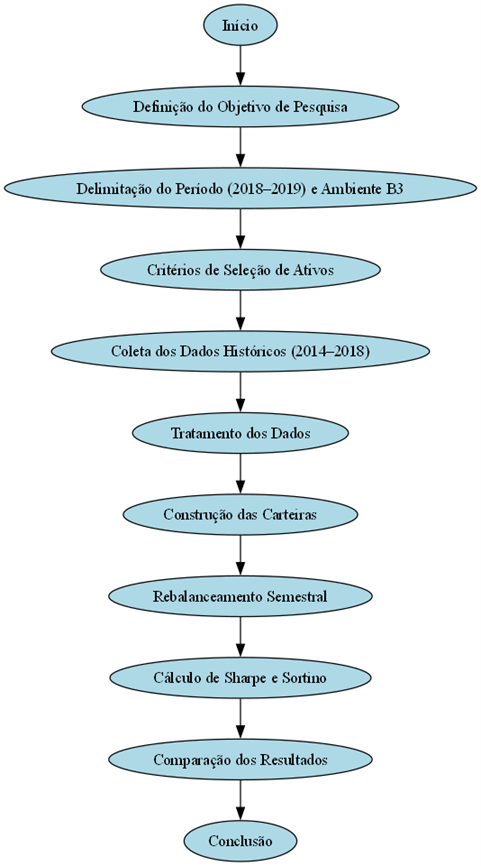
\includegraphics[width=0.8\textwidth]{image.png}
\caption{Fluxograma da Metodologia}
\textit{Fonte: Elaborado pelo autor.}
\label{fig:fluxograma_metodologia}
\end{figure}

\section{CRONOGRAMA DE ATIVIDADES}

A execução deste trabalho seguirá um cronograma estruturado em 6 meses, conforme apresentado na Tabela \ref{tab:cronograma}.

\begin{table}[h]
\centering
\caption{Cronograma de Atividades do TCC I (6 meses)}
\scriptsize
\begin{tabular}{|p{4.5cm}|*{6}{c|}}
\hline
\textbf{Atividades} & \textbf{M1} & \textbf{M2} & \textbf{M3} & \textbf{M4} & \textbf{M5} & \textbf{M6} \\
\hline
1. Revisão Bibliográfica e Referencial Teórico & X & X & & & & \\
\hline
2. Definição da Amostra de Ativos & X & & & & & \\
\hline
3. Coleta e Tratamento de Dados & & X & & & & \\
\hline
\quad • Extração de dados da base Economática & & X & & & & \\
\hline
\quad • Cálculo de retornos, volatilidades e covariâncias & & X & & & & \\
\hline
4. Implementação das Carteiras e Rebalanceamento & & & & X & & \\
\hline
\quad • Código Python (pandas, NumPy, cvxpy) & & & & X & & \\
\hline
\quad • Rebalanceamento semestral (jan e jul) & & & & X & & \\
\hline
5. Cálculo de Métricas e Análise Comparativa & & & & & X & \\
\hline
\quad • Sharpe e Sortino Ratio & & & & & X & \\
\hline
\quad • Gráficos e tabelas comparativas & & & & & X & \\
\hline
6. Redação de Resultados e Discussão & & & & & & X \\
\hline
7. Conclusão, Revisão Final e Entrega & & & & & & X \\
\hline
\end{tabular}
\normalsize
\label{tab:cronograma}
\end{table}

\section{LIMITAÇÕES DO ESTUDO}

Apesar do rigor metodológico adotado, este estudo apresenta algumas limitações que devem ser consideradas na análise dos resultados. Em primeiro lugar, não foram incorporados custos de transação, taxas, slippage e tributação nas operações de compra e venda dos ativos, o que pode gerar divergências entre os retornos simulados e os efetivamente obtidos na prática. Além disso, a utilização de séries históricas de retornos pressupõe que padrões passados se mantenham representativos para o futuro, o que pode não se confirmar em mercados sujeitos a choques exógenos e mudanças estruturais. Outra limitação refere-se à escolha de apenas três estratégias de alocação, desconsiderando alternativas mais recentes como o modelo de Hierarchical Risk Parity ou abordagens baseadas em Machine Learning, que poderiam trazer novas perspectivas. Por fim, a definição da taxa livre de risco como o CDI médio anualizado simplifica a realidade de investimentos no Brasil, que apresenta múltiplos instrumentos de renda fixa com diferentes graus de risco e liquidez. Tais limitações, embora não invalidem os resultados, indicam caminhos para aprofundamentos em pesquisas futuras.